\subsubsection{Backpropagation with Gradient Descent}
\label{sec:training-gradient-descent}
Due to the non-linearity in the network the minimum of the cost function cannot be computed analytically but numerically.
This is done using the gradient descent algorithm\cite{kiefer1952}\cite{robbins1951}.
\figref{fig:gradient-descent} illustrates this approach.
The cost function is evaluated and its gradients are computed using backpropagation\cite{rumelhart1986learning}.
The gradients point into the direction of steepest ascent.
Because a minimum needs to be found, those are negated for pointing into the direction of steepest descent.
Depending on these values representing the slope of the parameters, and, hence, their impact on the output, the parameters are changed to move closer to the minimum.
\begin{figure}
	\centering
	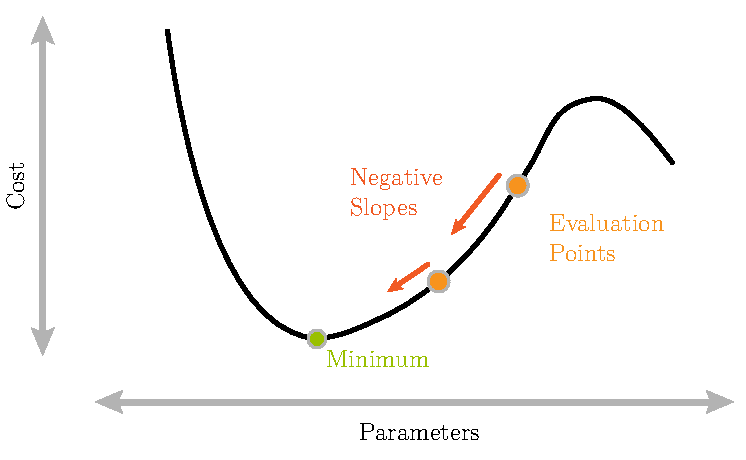
\includegraphics{images/gradient_descent.pdf}
	\caption[Schematic of Gradient Descent]{Schematic of gradient descent. Cost is evaluated, its negative gradients are computed and the parameters are moved along this direction until the minimum is reached.}
	\label{fig:gradient-descent}
\end{figure}
Following this approach means for the whole network that the cost function is backpropagated layer for layer to the beginning of the network using partial derivatives and the chain rule.
When this is completed, it is known how the parameters are influencing the output and therefore how they need to be changed depending on their slope.

Let's fill these statements with mathematical expression.
The goal of backpropagation is to compute the partial derivatives
\begin{subequations}
	\label{eq:backpropagation}
	\begin{align}
		\frac{\partial J}{\partial \vec{w}^{[l]}_{jk}}  = \frac{1}{m} \sum_{i}^{m} \frac{\partial J^{(i)}}{\partial \vec{w}^{[l]}_{jk}} \\
		\frac{\partial J}{\partial b^{[l]}_j} = \frac{1}{m} \sum_{i}^{m} \frac{\partial J^{(i)}}{\partial b^{[l]}_j}
	\end{align}
\end{subequations}
of the cost function w.r.t. the parameters by averaging the partial derivatives of cost functions of several samples.
The error of an neuron is defined by
\begin{equation}
	\delta^{[l]}_j = \frac{\partial J}{\partial a^{[l]}_j}
\end{equation}